\documentclass{article}

%%%%%%%%%%%%%%%%%%%%%%%%%%%%%%%%%%%%%%%%%%%%%%%%%%%%%%%%%%%%%%%%%
%package

%geometry
\usepackage[a4paper]{geometry}%调整页面边距
\geometry{left=3cm,right=3cm,top=3cm,bottom=3cm}
\linespread{1.5}
\usepackage{fancyhdr}%梦幻页眉

%fonts
\usepackage{fontspec}%字体库
\defaultfontfeatures{Mapping=tex-text}%启用tex风格字符		
\usepackage{xunicode,xltxtra}
\usepackage[BoldFont,SlantFont,CJKnumber,CJKchecksingle]{xeCJK}  % \CJKnumber{12345}: 一万二千三百四十五
\usepackage{CJKfntef}
\usepackage{bm} %公式中的粗体字符\boldsymbol
\usepackage{pifont}

%color
\usepackage{color,xcolor}
\definecolor{GREEN}{RGB}{25,180,68}
\definecolor{YELLOW}{RGB}{255,255,224}
\definecolor{BLUE}{RGB}{9,148,234}
\definecolor{RED}{RGB}{139,0,0}
\definecolor{DRED}{RGB}{128,0,0}
\definecolor{GREY}{RGB}{128,128,128}
\usepackage[pagecolor={YELLOW}]{pagecolor}%设置页面底色

%math
\usepackage{amsmath,amsfonts,amssymb}%必用宏包

%graphics
\usepackage[americaninductors,europeanresistors]{circuitikz}
\usepackage{tikz}%可以绘制各种坐标图,方格图
\usetikzlibrary{positioning,arrows,shadows,shapes,calc,mindmap,trees,backgrounds}  % placements=positioning
\usepackage{graphicx}%\includegraphics插图命令
\usepackage{subfigure}  %%图形或表格并排排列

% table
\usepackage{colortbl,dcolumn}  %% 彩色表格
\usepackage{multirow}%表格多行并列
\usepackage{multicol}%表格多列并列
\usepackage{booktabs}%创建没有竖线分隔的表格

% code
\usepackage{fancyvrb}%漂亮的代码包
\usepackage{listings}%加入代码

% ref
\usepackage{hyperref}%扩展参考文献,目录功能和加入超链接。

% title
\usepackage{titlesec}%花哨的章节标题

\usepackage{etoolbox}
\makeatletter
\patchcmd{\ttlh@hang}{\parindent\z@}{\parindent\z@\leavevmode}{}{}
\patchcmd{\ttlh@hang}{\noindent}{}{}{}
\makeatother%titlesec旧版本无编号问题


\titleformat
{\section} % command
[display] % shape
{\bfseries\Large} % format
{第\ \thesection 章\ } % label
{0.3ex} % sep
{
    \rule{\textwidth}{1pt}
    \vspace{1ex}
    \centering
} % before-code
[
\vspace{-2ex}%
\rule{\textwidth}{1pt}
] % after-code


%tightly-packed lists
\usepackage{mdwlist}
\usepackage{verbatim}%comment命令的注释包
\usepackage{styles/zhfontcfg}%中文包
\usepackage{styles/visionouclistings}
\usepackage{styles/visionouccfg}

% head/foot
\setlength{\headheight}{15pt}

\fancyhf{}



%%%%%%%%%%%%%%%%%%%%%%%%%%%%%%%%%%%%%%%%%%%%%%%%%%%%%%%%%%%%%%%%%%%%%%

%settings
\setCJKmainfont{Adobe Fangsong Std} %设置为楷体
\setCJKmonofont{Adobe Kaiti Std}%仿宋
%页眉页脚


\makeatletter
\def\headrule{{\if@fancyplain\let\headrulewidth\plainheadrulewidth\fi%
\hrule\@height 2.5pt \@width\headwidth\vskip1pt%上面线为2.5pt粗  
\hrule\@height 0.5pt\@width\headwidth  %下面0.5pt粗            
\vskip-2\headrulewidth\vskip-1pt}      %两条线的距离        
\vspace{6mm}}     %双线与下面正文之间的垂直间距              
\makeatother         
 

% graphics
\graphicspath{{figures/}}
\tikzset{
    % Define standard arrow tip
    >=stealth',
    % Define style for boxes
    punkt/.style={
           rectangle,
           rounded corners,
           draw=black, very thick,
           text width=6.5em,
           minimum height=2em,
           text centered},
    % Define arrow style
    pil/.style={
           ->,
           thick,
           shorten <=2pt,
           shorten >=2pt,},
    % Define style for FlyZhyBall
    FlyZhyBall/.style={
      circle,
      minimum size=6mm,
      inner sep=0.5pt,
      ball color=red!50!blue,
      text=white,},
    % Define style for FlyZhyRectangle
    FlyZhyRectangle/.style={
      rectangle,
      rounded corners,
      minimum size=6mm,
      ball color=red!50!blue,
      text=white,},
    % Define style for zhyfly
    zhyfly/.style={
      rectangle,
      rounded corners,
      minimum size=6mm,
      ball color=red!25!blue,
      text=white,},
    % Define style for new rectangle
    nrectangle/.style={
      rectangle,
      draw=#1!50,
      fill=#1!20,
      minimum size=5mm,
      inner sep=0.1pt,}
}

% code
\lstnewenvironment{VHDLcode}[1][]{%
  \lstset{
    basicstyle=\footnotesize\ttfamily\color{black},%
    columns=flexible,%
    framexleftmargin=.7mm,frame=shadowbox,%
    rulesepcolor=\color{blue},%
%    frame=single,%
    backgroundcolor=\color{yellow!20},%
    xleftmargin=1.2\fboxsep,%
    xrightmargin=.7\fboxsep,%
    numberstyle=\tiny\color{blue},%
    numberblanklines=false,numbersep=7pt,%
    language=VHDL%
    }\lstset{#1}}{}
\lstnewenvironment{VHDLmiddle}[1][]{%
  \lstset{
    basicstyle=\scriptsize\ttfamily\color{black},%
    columns=flexible,%
    framexleftmargin=.7mm,frame=shadowbox,%
    rulesepcolor=\color{blue},%
%    frame=single,%
    backgroundcolor=\color{yellow!20},%
    xleftmargin=1.2\fboxsep,%
    xrightmargin=.7\fboxsep,%
    numbers=left,numberstyle=\tiny\color{blue},%
    numberblanklines=false,numbersep=7pt,%
    language=VHDL%
    }\lstset{#1}}{}
\lstnewenvironment{VHDLsmall}[1][]{%
  \lstset{
    basicstyle=\tiny\ttfamily\color{black},%
    columns=flexible,%
    framexleftmargin=.7mm,frame=shadowbox,%
    rulesepcolor=\color{blue},%
%    frame=single,%
    backgroundcolor=\color{yellow!20},%
    xleftmargin=1.2\fboxsep,%
    xrightmargin=.7\fboxsep,%
    numbers=left,numberstyle=\tiny\color{blue},%
    numberblanklines=false,numbersep=7pt,%
    language=VHDL%
    }\lstset{#1}}{}
% pdf
\hypersetup{pdfauthor={Haiyong Zheng},%
            pdftitle={Title},%
            CJKbookmarks=true,%
            bookmarksnumbered=true,%
            bookmarksopen=false,%
            plainpages=false,%
            colorlinks=true,%超链接
            citecolor=green,%
            filecolor=magenta,%
            linkcolor=DRED,%red(default)
            urlcolor=cyan}
\newcommand\titlebar{%
\tikz[baseline,trim left=3.1cm,trim right=3cm] {
    \fill [cyan!25] (2.5cm,-1ex) rectangle (\textwidth+3.1cm,2.5ex);
    \node [
        fill=cyan!60!white,
        anchor= base east,
        rounded rectangle,
        minimum height=3.5ex] at (3cm,0) {
        \textbf{\thesection.}
    };
}%
}

%%%%%%%%%%%%%%%%%%%%%%%%%%%%%%%%%%%%%%%%%%%%%%%%%%%%%%%%%%%
%设置标题页面

\newcommand*{\titleGM}{\begingroup % 新命令:添加标题页
\hbox{ % 水平盒子
\hspace*{0.2\textwidth} % 左边空白
\rule{1pt}{\textheight\color{GREY}} % 竖线
\hspace*{0.05\textwidth} % 竖线和文本距离
\parbox[b]{0.75\textwidth}{ % 文本最大右边距

{\noindent\Huge\bfseries Git-GitHub \\[0.6\baselineskip] Getting Started}\\[4\baselineskip] % 题目
{\large \textit{Git-GitHub Manual of Vision Lab}}\\[5\baselineskip] % 标签或描述
{\Large \textsc{Jinna Cui}}\\ % 作者

\vspace{0.5\textheight} % 题目区域和作者间距
{\noindent August 2016 }\\[\baselineskip] % Publisher and logo
}}
\endgroup}


                      
\chead{\color{GREY}Git Manual}%页眉
\cfoot{\color{GREY}August 2016}%页脚 中
\lfoot{\color{GREY}Jinna}%页脚 左
\rfoot{\color{GREY}$\cdot$\ Page \thepage\ }%页脚 右
\renewcommand{\headrulewidth}{0.4pt}
\renewcommand{\footrulewidth}{0.4pt}

\usepackage{styles/lshort}

%%%%%%%%%%%%%%%%%%%%%%%%%%%%%%%%%%%%%%%%%%%%%%%%%%%%%%%%%%%%%%%%%
\begin{document}

\author{丁昊}%作者
\date{\vspace{-0.7em}2016年7月\vspace{-0.7em}}%日期
\titleGM\thispagestyle{empty}

\pagenumbering{roman}

\setcounter{page}{0}
\newpage
\begin{abstract}
Git是一种分布式版本控制系统,实验室主要用它来管理文档、代码等资料,所以学弟学妹们要学习Git 相关知识,并熟练使用Git 。本文参考孙雪师姐及郑老师《Git-GitHub-howto》文档,结合《git中文教程》及网上相关教程,围绕“为什么选择Git-GitHub”和“如何使用Git-GitHub”两个主题,对Git-GitHub做了详细却不冗余的介绍。由于是新手适用的Git攻略,本文更侧重基础知识,欢迎对Git的其他应用感兴趣的同学与我讨论,也欢迎大家批评指正!
\end{abstract}
\newpage

\tableofcontents 
\newpage

\pagestyle{fancy}

\pagenumbering{arabic}
\newpage
%%%%%%%%%%%%%%%%%%%%%%%%%%%%%%%%%%%%%%%%%%%%%%%%%%%%%%%%%%%%%%%%%
\section{Git \& GitHub}

\subsection{什么是Git}
在理解Git之前,首先要理解版本控制系统的概念。版本控制系统是用来记录文件内容变化以便查阅版本修改情况的系统。用大家都经历过的毕业论文举例,写论文要经过很多次的修改,我们惯用的是每次修改之前将前一版本复制到本地,备份好之后,再修改文件名以示区分:论文1,论文2……论文final,论文final1……论文finalfinal……往往一篇论文结束,本地备份几十次,这就是本地版本控制系统。如果文件很大,这样的备份方式对内存来说,也是一种挑战。有的同学会将备份上传到中央服务器,这属于集中化的版本控制系统,而中央服务器一旦宕机,丢失数据的风险很大。除此之外,这两种版本控制系统最大的缺陷在于:无法直观的看到版本与版本之间的不同,系统并没有对修改过的地方清晰地标注。这些问题都可以用Git来解决。Git属于分布式版本控制系统,在Git中,本地仓库将远程仓库的文件完整地镜像下来(如图1),这样任何一处服务器发生故障,事后都可用本地仓库恢复。除此之外,Git管理文件时,可清晰地看到版本更新时内容的变化,可恢复任意版本。这对文件管理尤其代码管理有重要意义。

\begin{figure}[!htb] %插图
\centering 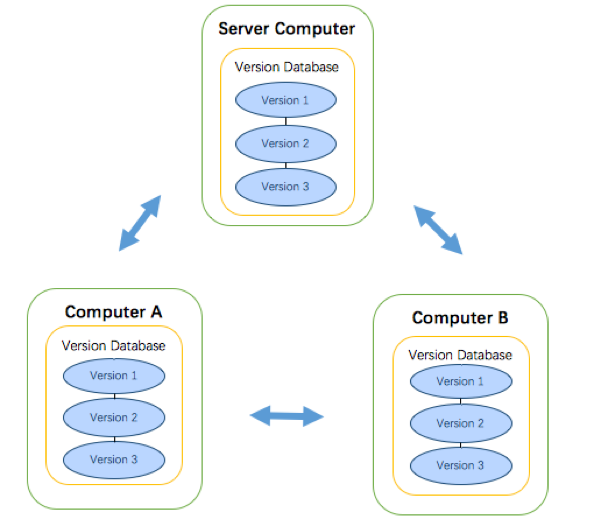
\includegraphics[width=0.5\textwidth]{fig1.png} \caption{分布式版本控制系统}
\label{fig:1}
\end{figure}

\subsection{什么是GitHub}

GitHub是利用Git进行版本控制,用于代码托管的共享虚拟主机服务。Github上可以创建私人仓库和公共仓库,创建私人仓库需付费,这也是GitHub的优点所在,公共仓库可以很方便的进行分享和协作。举个例子,A新建一个公共仓库,上传自己的代码,其他人都可以看到,大家可以一起讨论,提问等。如果B发现A的代码有问题,可以用\textbf{Issues}选项向A提出他代码中的问题,如果B对这部分代码有更好的建议,可以写出来,通过\textbf{Pull requests}选项向A提交自己的编码,如果A认为B的方案确实不错,A将会把B贡献的代码融合到自己的代码中。这为代码分享和分工合作提供了极大的便利。



\section{设置SSH密钥}
Git可以通过四种协议来传输数据:本地传输,SSH协议,Git 协议和HTTP协议。下面介绍如何通过SSH协议来使用Git。关于服务器上Git协议的问题,请参考:\url{https://git-scm.com/book/zh/v1/}4.1节,在此不再赘述。SSH(Secure Shell)是建立在应用层和传输层基础上的安全协议,为计算机上的Shell提供安全的传输和使用环境。简言之,SSH负责保护本地仓库和远程仓库之间数据传输时不被截获。

\subsection{生成密钥}
打开终端,在~目录下执行\textbf{ssh-keygen -t rsa}。中间会出现enter passphrase的指令,此处一直按enter键即可。执行完之后,在.ssh文件中已生成了id \_ rsa.pub文档。此时,执行\textbf{ls -a},可见名为.ssh的隐藏文件,执行\textbf{cd .ssh},转到.ssh文件夹,再执行\textbf{ls}指令便可看到该目录下已生成的名为id \_ rsa.pub文件。

\subsection{把公共密钥保存到GitHub网站上}
浏览器打开网页\url{http://www.github.com},注册(sign up)自己的github账号之后登陆(sign in),点击settings,选择SSH and GPG keys 选项,点击New SSH key,title写为:your name@iplouc(如图2),打开id\_rsa.pub(在.ssh文件夹展开看到id\_rsa.pub,执行 vim id\_rsa.pub指令,便可读取id\_rsa.pub中的内容),将里面的内容复制到key中,然后保存即可。

\begin{figure}[!htb] %插图
\centering 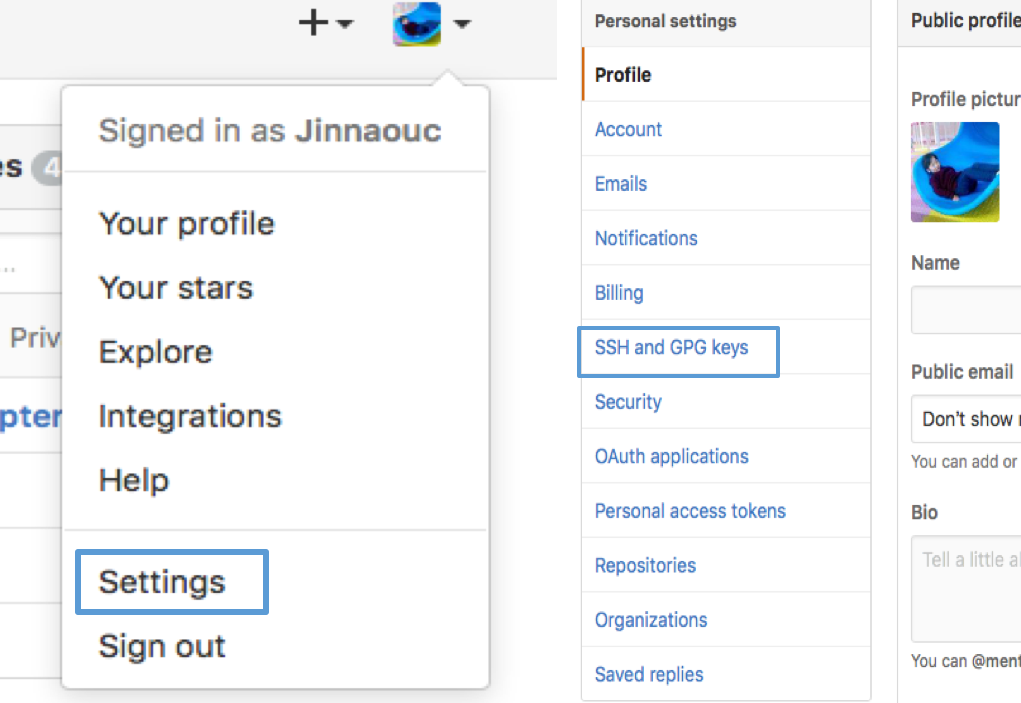
\includegraphics[width=0.5\textwidth]{fig2.png} \caption{进入SSH keys 设置界面}
\label{fig:1}
\end{figure}

\subsection{将密钥加载到SSH里}
执行 \textbf{ssh-add}即可。

\newpage
\section{Git的安装与配置}
本章的主要内容是:基于Ubuntu 16.04 系统,Git的安装与配置。

\subsection{下载与安装}
执行\textbf{sudo apt-get install git},便可完成Git的下载,这个过程有点慢,耗时多少一定程度上取决于网速和人品。

\subsection{初次运行Git前的配置}
在初次运行Git 前,要设置个人的用户名和电子邮件地址,Git提交时会引用用户名和电子邮箱地址来说明是谁提交了更新,git config是专门用来对Git进行配置的指令,我们用git config来设置用户名和密码。执行以下指令:

\textbf{git config {-}{-}global user.name “your name”}

\textbf{git config {-}{-}global user.email “your email”}

注:双引号部分填写个人用户名和email地址,不要忘记双引号。设置完成后,执行\textbf{git config {-}{-}list }指令,便可查看是否设置成功。

\section{Git的基础使用}

本章主要对Git基本使用做了详细的讲解,其中*号部分在第一次练习使用github时可先不练习,因为其中涉及到一些删除,撤销等问题,刚开始使用Git可能不太熟悉。待学会基础Git的基础使用之后,可练习*部分。

\subsection{克隆远程仓库}
首先,在你的GitHub上新建一个repository,命名为gittest(如图3), 设置好之后,点击Create repository。此时,便已新建一个名为gittest的仓库。

\begin{figure}[!htb] %插图
\centering 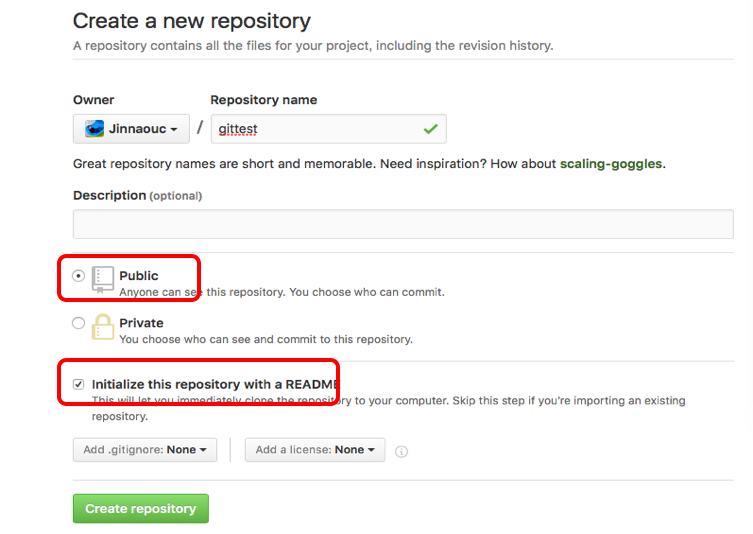
\includegraphics[width=0.5\textwidth]{fig3.png} \caption{新建仓库}
\label{fig:1}
\end{figure}

进入gittest仓库之后,在红框部分可看到gittest仓库的ssh地址(如图4)。

\begin{figure}[!htb] %插图
\centering 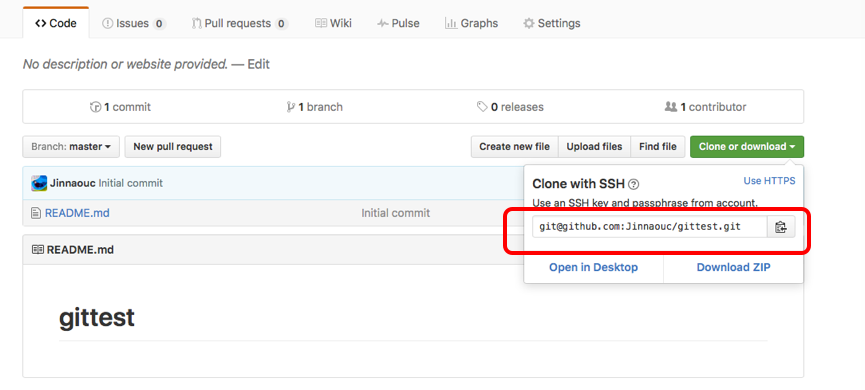
\includegraphics[width=0.5\textwidth]{fig4.png} \caption{复制仓库地址}
\label{fig:1}
\end{figure}

执行 \textbf{git clone git@github.com:Jinnaouc/gittest.git},记得改成自己的ssh地址。此时,在当前目录下用ls指令查看,便可看到本地目录有了一个名为gittest的文件夹,进入这个文件夹,用ls 命令可查看,此文件夹中只有一个README.md文件。

*删除仓库:有些仓库我们创建之后,不想要了,比如此次创建的gittest仓库,以后不想让它再留在自己的GitHub中,可将该仓库删除。在自己的GitHub主页上,进入gittest仓库后点击\textbf{Settings}选项(如图5),将该页面拉至最下方,找到\textbf{Delete this repository},点击后并输入当前仓库名确认后,便可将该仓库删除。
 \begin{figure}[!htb] %插图
\centering 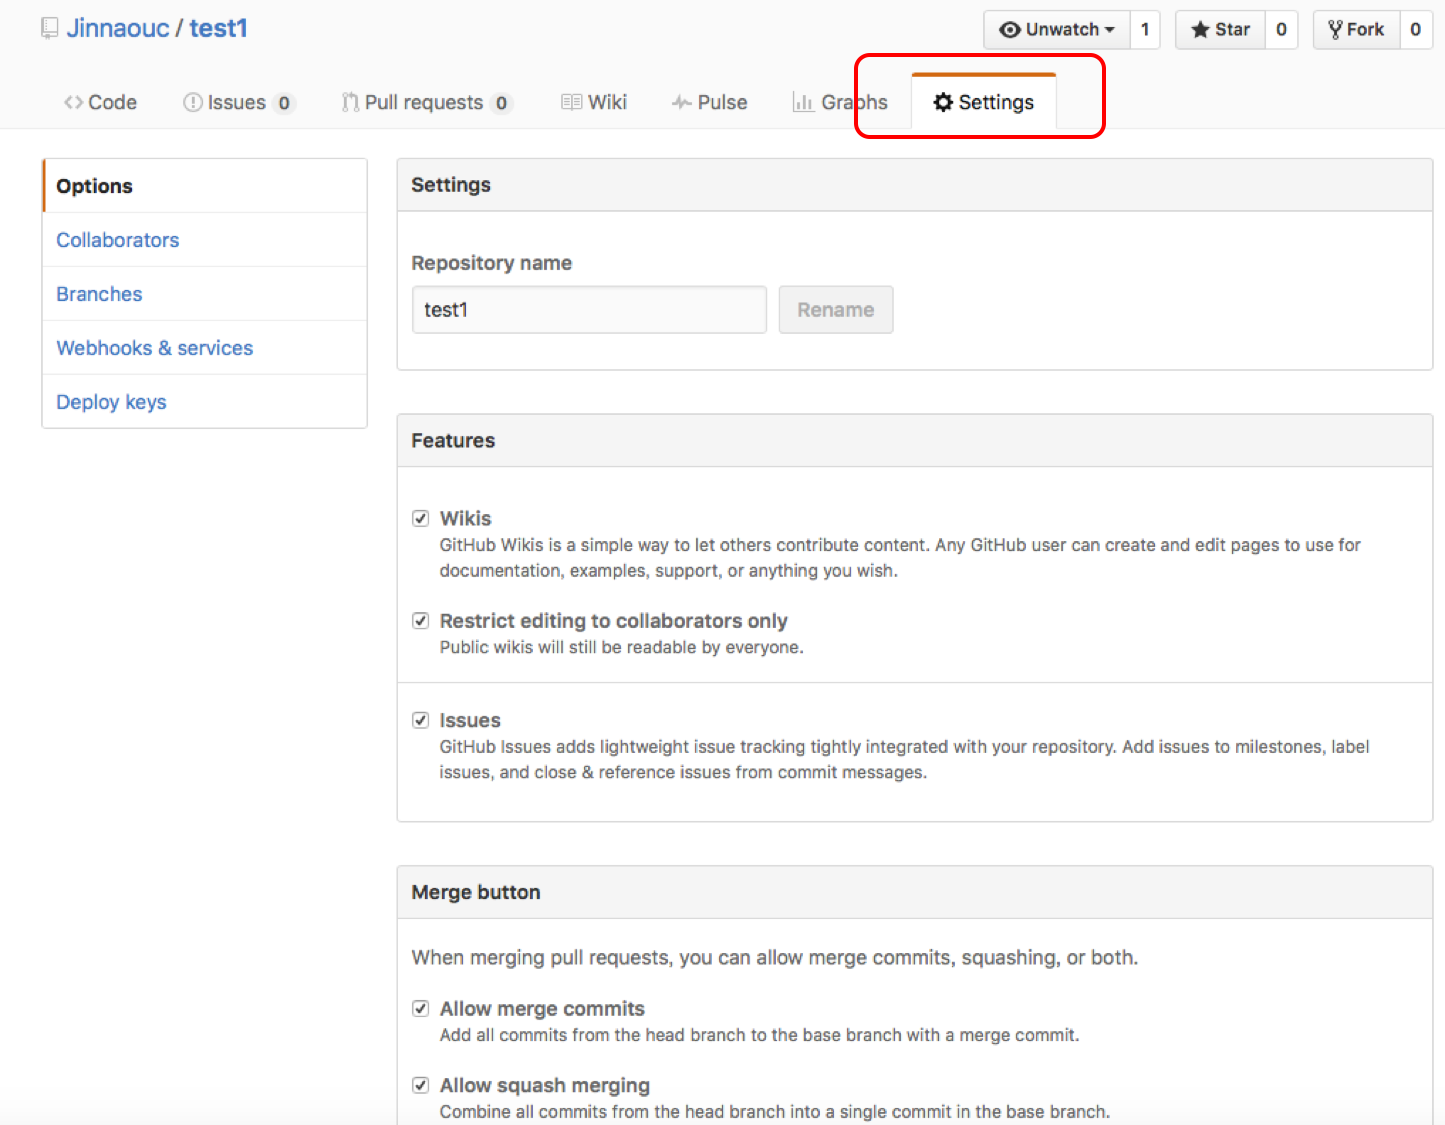
\includegraphics[width=0.5\textwidth]{fig5.png} \caption{进入仓库设置}
\label{fig:1}
\end{figure}

\begin{figure}[!htb] %插图
\centering 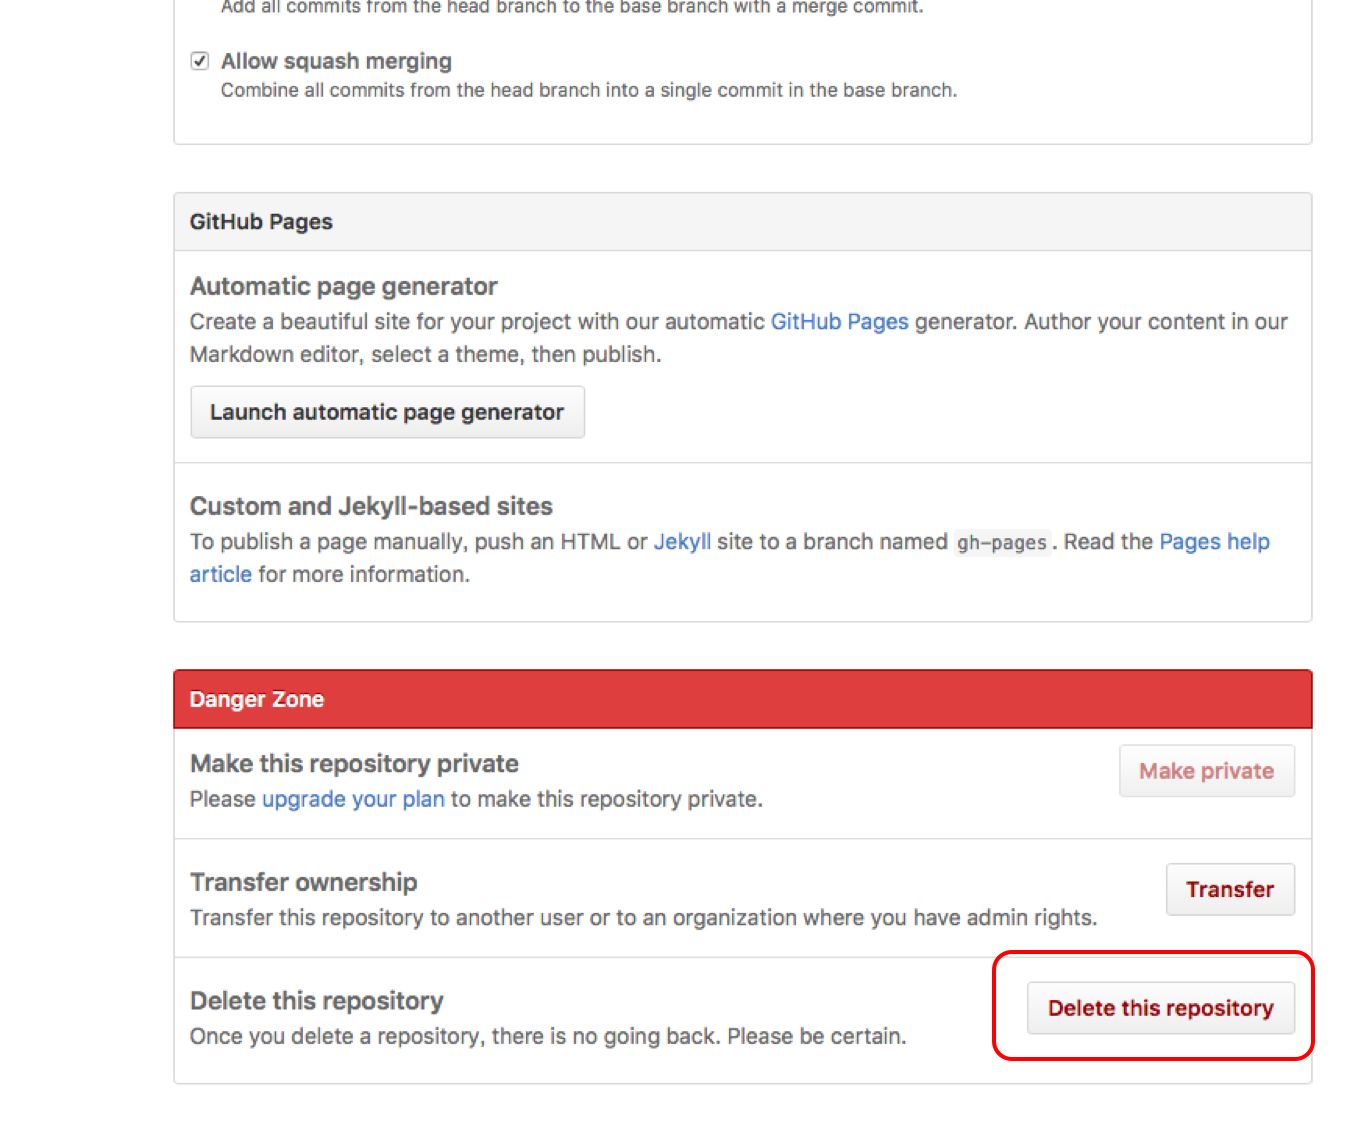
\includegraphics[width=0.5\textwidth]{fig6.png} \caption{点击删除仓库}
\label{fig:1}
\end{figure}

\subsection{初始化仓库}
进入gittest文件夹后,在此目录下初始化仓库。执行\textbf{git init} 初始化仓库之后,在当前Git Test目录下,已生成名为.git的隐藏工作目录,通过指令 ls -a 查看,一定要确认.git文件已生成。这一步非常重要,以后所有Git需要的数据和资源都存放在这个目录中。

\subsection{文件提交}
工作目录中的文件的两种状态:已跟踪或未跟踪。已跟踪的文件是指已经纳入版本控制管理的文件,它们可以进行修改,暂存,提交等操作。接下来,以文档“hello”为例,详细说明文件提交的过程。
\subsubsection{新建hello文档}
执行\textbf{touch hello}。
\subsubsection{在文档中写入内容}
执行\textbf{vim hello}指令,打开vim编辑界面,按i,o,a,r(不区分大小写)四个字母在进入编辑界面后输入 Hello! ,按esc键,输入 :wq(保存退出指令)即可。也可再次在目录终端下输入 vim hello 确认是否编辑成功。
\subsubsection{查看当前文件状态}
git status 命令可以查看文件在任何时候的状态。执行\textbf{git status} 可以看到,此时跟踪状态显示为存在未跟踪的文件。



\subsubsection{开始跟踪}
执行\textbf{git add hello},执行完此条指令之后,hello便已被跟踪且切换为暂存(staged)状态,正式纳入Git的控制系统。此时可再次使用 git status指令查看。

*也可以尝试使用\textbf{git add .}和\textbf{git add  *}指令,二者都可自动将当前目录\textbf{所有}修改过的文件跟踪,但有时会有一些自动生成的文件,无需纳入Git的管理,这会将本无需提交的文件也一起纳入Git管理。



\subsubsection{查看修改文件}
再次执行\textbf{vim hello},将其内容改为 hello world! 保存后退出。此时,执行\textbf{git diff},便可以查看文档的具体修改内容(添加和删除的行)。

*取消修改:执行\textbf{git checkout {-}{-}hello}指令,执行之后可再次使用git diff指令查看,便可发现已没有修改情况,即对hello的修改已撤消。
\subsubsection{跟踪修改文件}
此时在目录终端下执行 \textbf{git status}查看hello文档的状态。可发现,此时出现了两个状态:原hello文件依然是已暂存状态,修改后的hello文件是未暂存状态。需再次使用\textbf{git add hello}指令来暂存已更改的hello文档。也就是说,每次对文档进行修改之后,都要用git add指令提交暂存。此时,若要查看已暂存文档与上次提交的文档中不同的内容,可执行 \textbf{git diff --cached}命令,此时可以查看已暂存的修改文件和原文件的差异。注意:此时文档已暂存,用git diff 命令看不到任何修改信息,这两条命令要注意区分。

*取消跟踪:执行\textbf{git rm {-}{-}cached hello},此时再用git status指令查看hello的状态,此时hello的状态则变成了未跟踪即文件便已从暂存区移除。

*移除已暂存文件:执行\textbf{git rm hello -f}强制删除已暂存的hello文档,这条命令可将hello文档彻底删除。

*忽略未跟踪文件:在编译过程中,可能会产生一些不需要纳入Git管理的文件(通常为隐藏文件),此时我们可以将这些文件忽略,被忽略的文件将不会提交到Git。首先确保需要忽略的文件是未跟踪状态,如果已跟踪,请用取消指令取消跟踪。然后在项目仓库下创建.gitignore文件:\textbf{touch .gitignore},写入要忽略的文件的扩展名,例如,想要忽略所有.DS\_Store文件,则写入  \textbf{*.DS\_Store },保存退出即可。

\subsubsection{提交文件}
我们平时更多采用-m参数来直接提交文件及文件说明。执行 \textbf{git commit -m `message'},即可直接提交文档hello。在这个语句中,git commit是提交文件的指令,`message'是说明,可自行更换。大家可以新建一个hello2文档,尝试在跟踪后,用\textbf{git commit}指令直接提交。这种提交方式会启动一个文本编辑器来用于提交说明,开头有一空行供你输入说明。此时的说明可以为空,也可以自行定义。提交之后,再次查看跟踪状态可发现已没有需要更新的文件。提交前要检查文件的跟踪状态,尤其修改的,新建的文件,要检查是已暂存了。此时,已经完成了第一步:将文件更新到本地仓库。

*跳过使用暂存区域:使用暂存区域的方式可以精心准备和检查待提交的文件,但是有时候却会非常繁琐,Git提供了一个跳过使用暂存区域的方式,直接 执行\textbf{git commit -a -m `message'}即可直接提交。 

*查看提交历史:执行\textbf{git log}指令,可以看到以提交时间为顺序的所有更新, 若执行\textbf{git log -p -2}指令可以显示最近两次的更新;\textbf{git log --stat} 指令可以简要显示增加和删除的行数。执行\textbf{git log {-}{-}since=2.weeks}指令可以显示两周内的提交情况。除此之外,git log指令还有其他有趣的应用,具体可参考《git 中文教程》 第27页。


\subsection{推送数据到远程仓库}
\subsubsection{查看当前远程库}
执行 \textbf{git remote -v}指令,可查看当前配置的远程库,此时可以看到,默认的库名为origin,若执行\textbf{git remote}指令,则只能看到远程库名称,不能看到具体的仓库地址。

*执行\textbf{git remote show origin}可以查看origin这个远程仓库的详细信息。

\subsubsection{抓取数据}
执行\textbf{git fetch origin},将仓库最新更新的数据抓取到本地,有的人习惯使用\textbf{git pull}命令,pull和fetch的区别在于:pull不仅可以抓取数据,还能合并分支(分支的相关问题可参考\url{https://git-scm.com/book/zh/v2}第三章Git分支部分,在此不再赘述)。fetch和pull命令与克隆命令的区别在于,它们只到远程仓库拉取所有本地仓库中没有的数据。其重要性将在3.4节最后实验室应用部分解释。

*添加远程仓库:在自己的github主页新增一个仓库,git remote add [名称] [地址],执行 \textbf{git remote add public git@github.com:Jinnaouc/D.git},记得改成自己新仓库的地址。其中,public是新仓库的名字,因为原仓库已默认名称为origin,再次添加仓库的时候,必须输入仓库名,并且每次添加的仓库名称不能重复,否则无法添加。仓库添加后,可执行 \textbf{git fetch public}来从新的仓库中抓取数据。

*远程仓库重命名: git remote rename [原名] [新名] 执行 \textbf{git remote rename origin report},这样便将原名为origin的仓库更名为report,可用git remote -v 再看下远程仓库配置信息。
\subsubsection{推送数据至远程仓库}
执行 \textbf{git push origin master},此时,你的hello文档已经push到github的gittest仓库了,可登录github查看。其中,origin为默认的仓库地址名称,master为默认的分支名称,在未自行设定仓库地址名称和分支名称前,系统使用默认名称,在github操作扩展部分(此处加超链接),会具体讲到如何修改名称,若名称修改后,指令也要对应修改。

\subsubsection{恢复历史版本}

在对文件进行修改之后,如果要恢复到以前的某个版本,Git 也可以实现。首先执行\textbf{git log}指令,可查看提交历史,每个提交历史commit 之后都有其对应的哈希值(由40个16进制字符0-9及a-f组成),例如1d755b5ce673d582dcff067120b347f47ca6a6c3。选定你要回到哪个版本,复制下该版本的哈希值后退出。git reset 命令有很多参数选项,现只介绍用来恢复历史版本的hard和soft选项。执行\textbf{git reset {-}{-}hard hash},其中,hash 要改为刚刚复制的哈希值。执行完该命令后,已将历史版本恢复。注意:选用hard选项恢复历史版本会删除此版本之后的所有提交更新的版本。恢复之后,要重新更新到远程GitHub上,执行\textbf{git push -f origin master}即可。记住,-f参数意为强制执行,必不可少,此时如果不强制执行,会提示使用git pull命令将远程项目合并到本地,造成混乱。若要恢复单个文件的历史版本,可以执行\textbf{git log filename}来查看文件版本的哈希值,仍使用\textbf{git reset {-}{-}hard hash}

\section{实验室Git-GitHub的使用}
相信你已经学会了如何将本地仓库的文件上传到了自己的github新建的仓库中,接下来对实验室的Git的使用,给大家做一个简单的介绍。实验室的Git网址:\url{https://github.com/zhenglab},点击进入之后,可以看到,有很多老师创建的仓库,从仓库克隆文件不需要权限,直接执行克隆命令,将你想要的文件克隆到本地即可。若推送数据到仓库,则需要老师授予权限,有了权限之后,才可向仓库中推送数据,push的方式和向自己Git 仓库中push的方式一样。注意,与推送数据到自己的仓库不同的是,向仓库中推送数据的可能不止自己一个人,如果在你推送数据之前,其他人已经推送了若干更新,你的推送将被驳回,必须先把他们的更新抓取到本地,再推送自己的项目,这便是执行4.4.2命令的必要性。总结:向仓库推送数据,首先要获得权限,其次要确保无人更新或已将最新更新抓取到本地。

\section{总结}

以上就是对Git的基础应用的总结,本文是我整理了孙雪师姐和郑海永老师之前的文档,结合相关教程总结出来的。由于身边人对Git的使用均有一定的掌握,因此,没有进行很好的测试。这份攻略是否非常适用毫无经验的新生,还需要接受未来学弟学妹们的考验。同时,非常欢迎大家提出批评意见和补充意见!


\end{document}
